\subsection{Quasi-Galois extensions}

DEFINITION 2. --- Let E be an extension of K. Then E is said to be quasi-Galois or normal (over K), if it is algebraic and if every irreducible polynomial of K{[}X{]} which has at least one root in E, splits into a product of polynomials of degree 1 (distinct or not) in E{[}X{]}.

If E is an algebraic closure of K, it is a quasi-Galois extension of K; for the condition (AC) of Prop. 1 (V, p.~19) asserts that every non-constant polynomial in E{[}X{]} is a product of polynomials of degree 1.

PROPOSITION 3. --- Let E be an extension of K contained in Ω. Then the following conditions are equivalent :

\begin{enumerate}
\def\labelenumi{\alph{enumi})}
\item
  E is a quasi-Galois extension of K.
\item
  For each \(x \in \mathbf{E}\) the conjugates of \(x\) over \(\mathbf{K}\) in \(\Omega\) all belong to \(\mathbf{E}\) .
\item
  Every K-automorphism of \(\Omega\) maps the field E into itself.
\item
  Every K-homomorphism of E into \(\Omega\) maps E into itself.
\item
  E is the splitting extension in \(\Omega\) of a family \((f_i)_{i\in I}\) of non-constant polynomials in K{[}X{]} (V, p.~24, Remark 3).
\end{enumerate}

The equivalence of c) and d) stems from the fact that every K-homomorphism of E into \(\Omega\) is induced by a K-automorphism of \(\Omega\) (V, p.~52, Prop. 1).

By definition a quasi-Galois extension is the splitting field of the family of minimal polynomials (over K) of its elements, so \(a\) implies \(e\) ). Under the hypothesis \(e\) let \(u\) be an automorphism of \(\Omega\) ; for each \(i \in I\) , \(u\) permutes the set \(\mathbf{R}_i\) of roots of \(f_i\) and since \(\mathbf{E} = \mathbf{K}\left(\bigcup_{i \in I} \mathbf{R}_i\right)\) , we have \(u(\mathbf{E}) = \mathbf{E}\) ; thus \(e\) implies \(c\) .

The definition of conjugate elements shows that \(c)\) implies \(b)\) . Finally assume that \(b)\) holds; let \(f\) be a monic irreducible polynomial in \(K[X]\) having at least one root \(x\) in \(E\) ; since \(\Omega\) is algebraically closed, there exist elements \(a_k\) of \(\Omega\) ( \(1 \leqslant k \leqslant n\) ) such that \(f(x) = \prod_{k=1}^{n} (X - a_k)\) and since the \(a_k\) are the conjugates of \(x\) over K (V, p.~53, Cor. 1), they belong to E by hypothesis. So we have shown that b) implies a).

COROLLARY 1. --- For an extension E of K contained in Ω to be quasi-Galois it is necessary and sufficient that it should be identical to all its conjugates over K.

This follows from Prop. 1, a) (V, p.~52) and the equivalence of the conditions \(a\) and \(c\) of Prop. 3.

COROLLARY 2. --- Let E and F be two algebraic extensions of K such that \(E \subset F\) . If F is quasi-Galois over K, then it is quasi-Galois over E.

We may assume that \(F \subset \Omega\) . Let u be an E-automorphism of \(\Omega\) . Since u is a K-automorphism of \(\Omega\) and F is quasi-Galois over K, we have \(u(F) = F\) , therefore F is quasi-Galois over E.

COROLLARY 3. --- Let N be a quasi-Galois extension of K contained in \(\Omega\) , and E a subextension of N. Let u be a K-homomorphism of E into \(\Omega\) ; then \(u(E) \subset N\) and there exists a K-automorphism v of N which induces u on E.

Let w be a K-automorphism of \(\Omega\) extending u (V, p.~52, Prop. 1); since N is quasi-Galois over K, we have \(w(\mathbf{N}) = \mathbf{N}\) , whence \(w(\mathbf{E}) \subset \mathbf{N}\) and so w induces a K-automorphism v of N.

COROLLARY 4. --- Let E' be an extension of K and E, K' two subextensions of E'. Suppose that E is quasi-Galois over K and E' = K'(E) ; then E' is quasi-Galois over K'.

Let \((f_i)_{i\in I}\) be a family of non-constant polynomials in \(\mathbf{K}[\mathbf{X}]\) whose splitting field over \(\mathbf{K}\) is E. Then it is clear that \(\mathbf{E}'\) is the splitting field of the family \((f_i)_{i\in I}\) over \(\mathbf{K}'\) , so it is quasi-Galois over \(\mathbf{K}'\) .

Remarks. --- 1) Let F be an extension of K and E a subextension of F, and suppose that E is quasi-Galois over K. Let us show that every K-automorphism u of F leaves E invariant. For let \(x \in E\) and f the minimal polynomial of x over K. Since E is quasi-Galois over K, there exist \(a_{1}, \ldots, a_{n} \in E\) such that \(f(\mathbf{X}) = \prod(\mathbf{X} - a_{i})\) ; we have \(f(u(x)) = u(f(x)) = 0\) , hence \(u(x)\) is one of the \(a_{i}\) and so belongs to E. We have proved \(u(\mathrm{E}) \subset \mathrm{E}\) , and now \(u(\mathrm{E}) = \mathrm{E}\) follows by V, p.~52, Prop. 1.

\pandocbounded{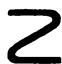
\includegraphics[keepaspectratio]{images/part001_36e9f8fa.jpg}}

\begin{enumerate}
\def\labelenumi{\arabic{enumi})}
\setcounter{enumi}{1}
\item
  Suppose that E is a quasi-Galois extension of K and F a quasi-Galois extension of E; it is not always the case that F is quasi-Galois over K (V, p.~153, Ex. 1). The reason is the following: let u be a K-automorphism of \(\Omega\) ; we have \(u(E) = E\) , but if f is the minimal polynomial over E of an element x of F, it is not necessarily invariant under u; therefore \(u(x)\) is not necessarily conjugate to x over E, and so need not necessarily belong to F. In that case F and \(u(F)\) are two distinct quasi-Galois extensions of E which are K-isomorphic but not E-isomorphic.
\item
  Let E be an algebraic extension of K and x, y two elements of E. If there exists a K-automorphism of E which maps x to y then x and y have the same minimal polynomial over K and so are conjugate over K by Prop. 2 (V, p.~52). The converse holds if E is quasi-Galois, because every K-automorphism of \(\Omega\) induces a K-automorphism of E. The hypothesis that E be quasi-Galois is not superfluous as the following example shows: let K = Q and \(\Omega\) the field of all algebraic numbers; put \(E = \Omega \cap R\) . It may be shown (V, p.~153, Ex. 2) that every automorphism of E is the identity mapping and that \(\sqrt{2}\) and \(-\sqrt{2}\) are elements of E conjugate over Q.
\end{enumerate}

